% Created 2021-07-17 Sat 12:29
\documentclass[11pt]{article}
\usepackage[utf8]{inputenc}
\usepackage[T1]{fontenc}
\usepackage{fixltx2e}
\usepackage{graphicx}
\usepackage{longtable}
\usepackage{float}
\usepackage{wrapfig}
\usepackage{soul}
\usepackage{textcomp}
\usepackage{marvosym}
\usepackage{wasysym}
\usepackage{latexsym}
\usepackage{amssymb}
\usepackage{hyperref}
\tolerance=1000
\providecommand{\alert}[1]{\textbf{#1}}

\title{README}
\author{}
\date{\today}
\hypersetup{
  pdfkeywords={},
  pdfsubject={},
  pdfcreator={Emacs Org-mode version 7.9.3f}}

\begin{document}

\maketitle

\setcounter{tocdepth}{3}
\tableofcontents
\vspace*{1cm}
\section{The USB Gadget and the Pi}
\label{sec-1}

Does this work?
\subsection{This iPad}
\label{sec-1-1}

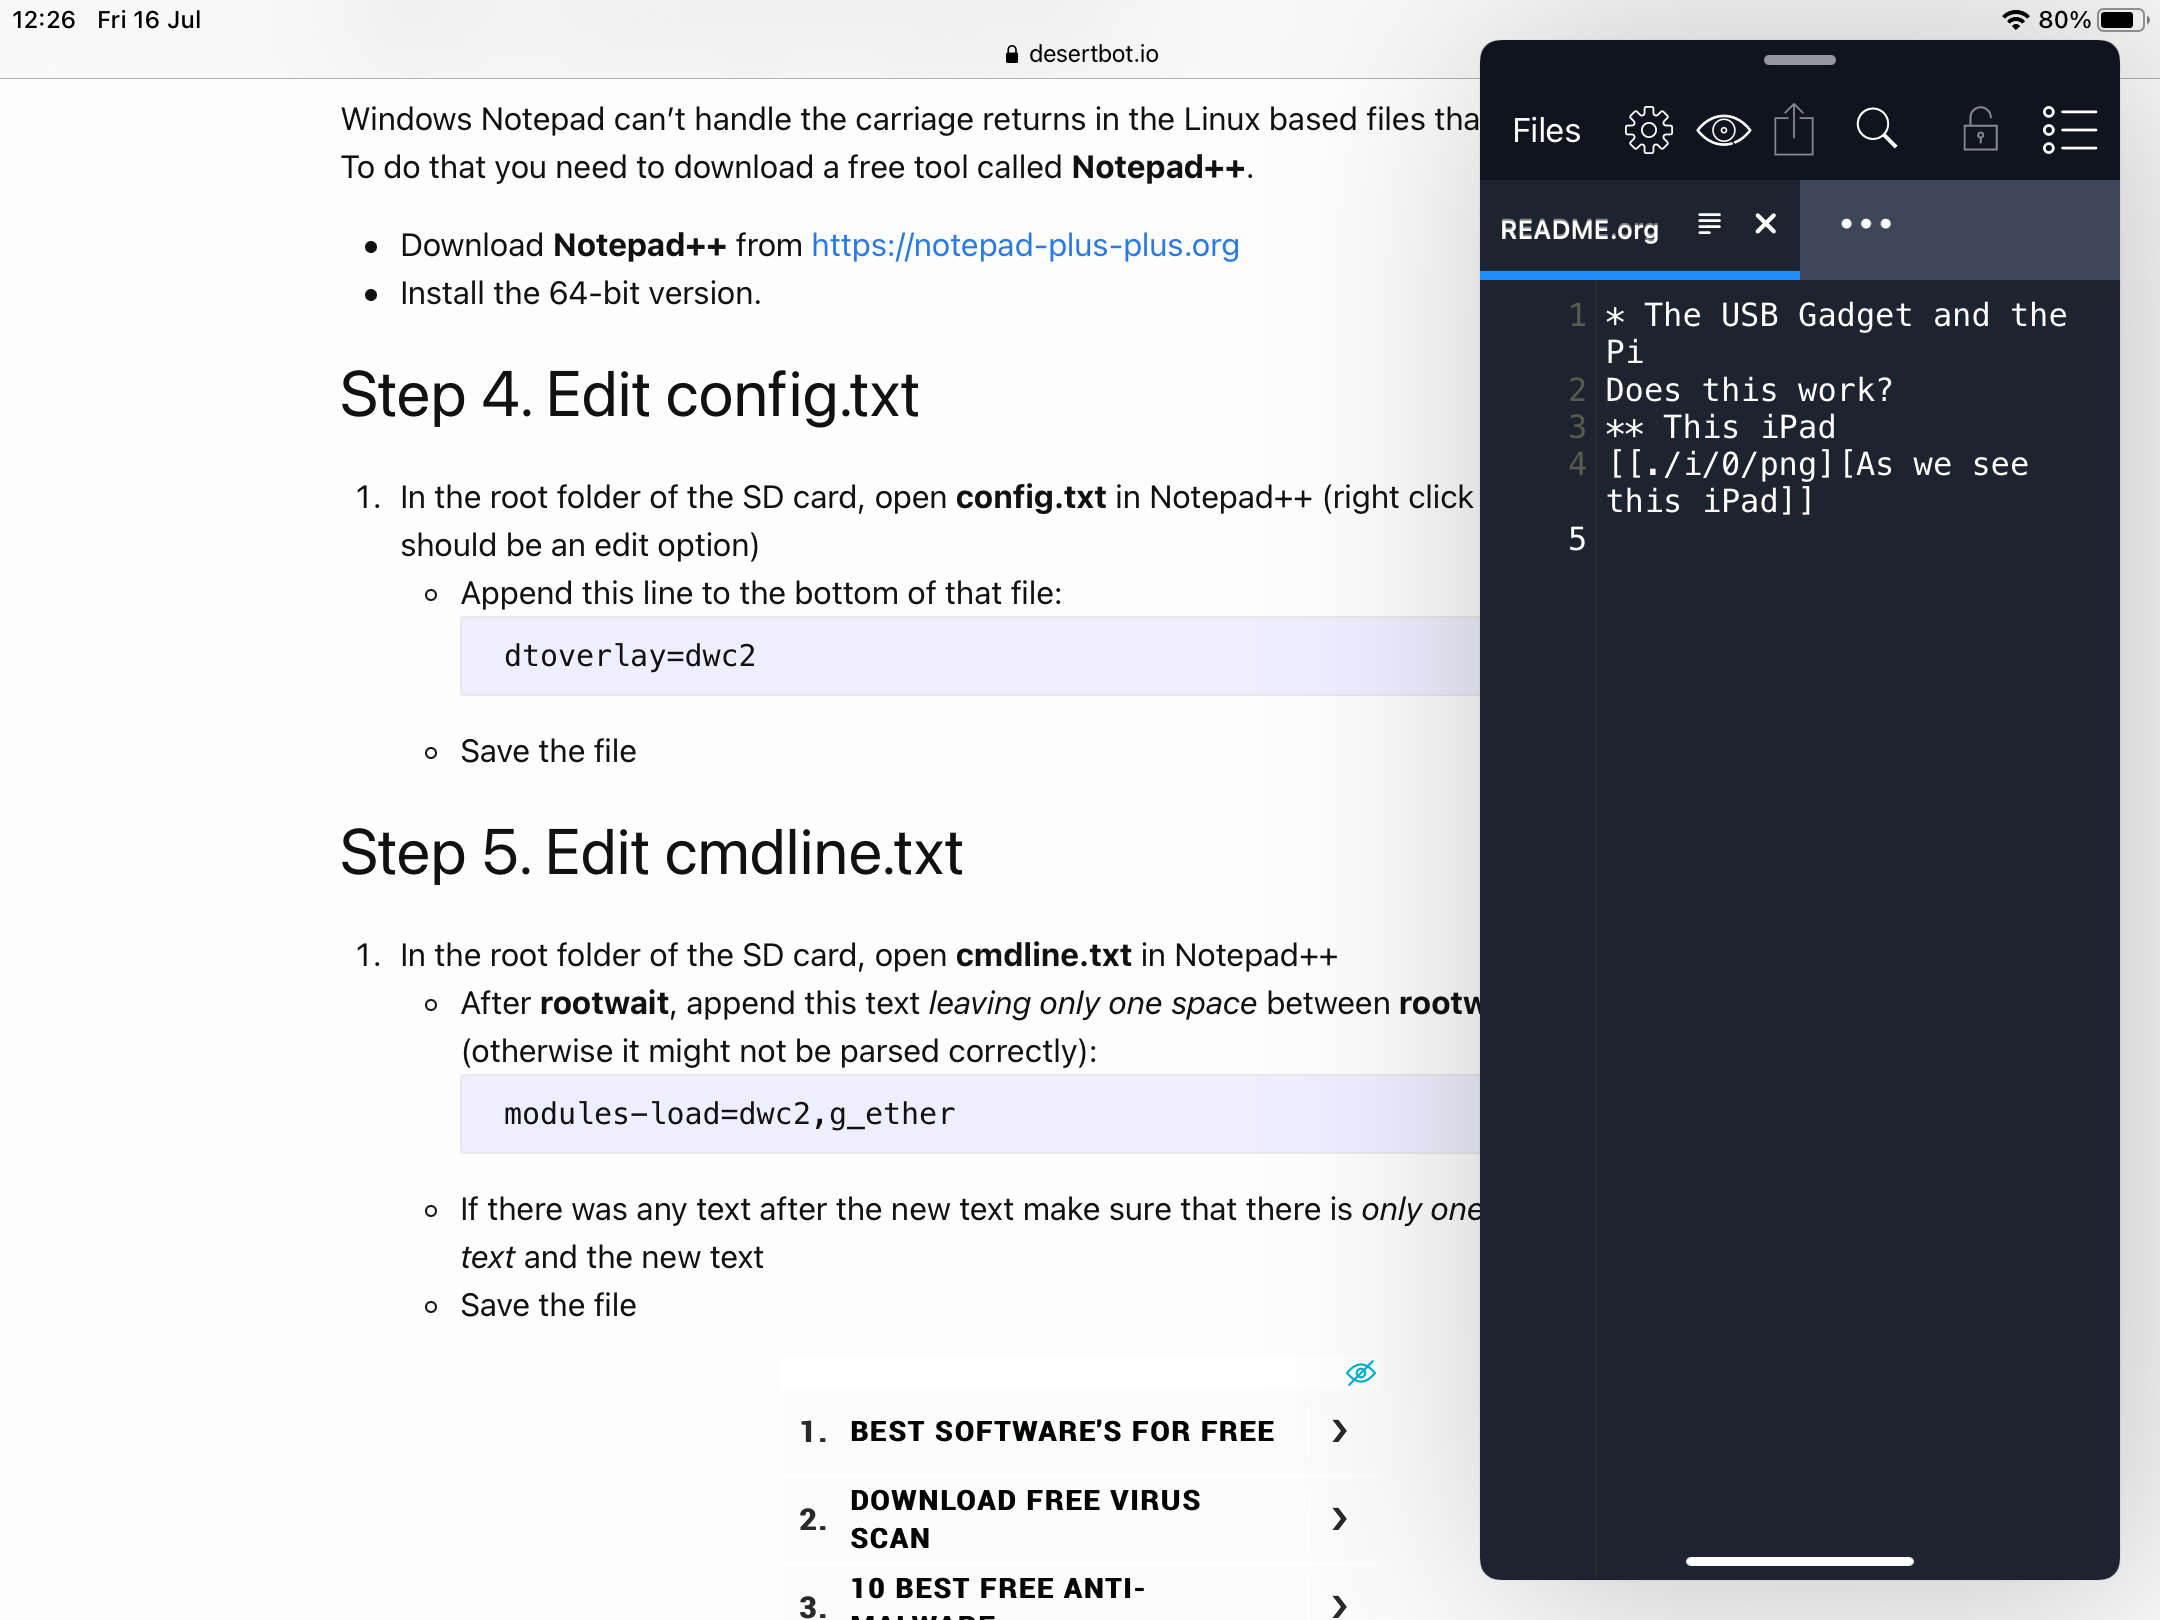
\includegraphics[width=.9\linewidth]{./i/0.png}
\subsection{Things for this}
\label{sec-1-2}

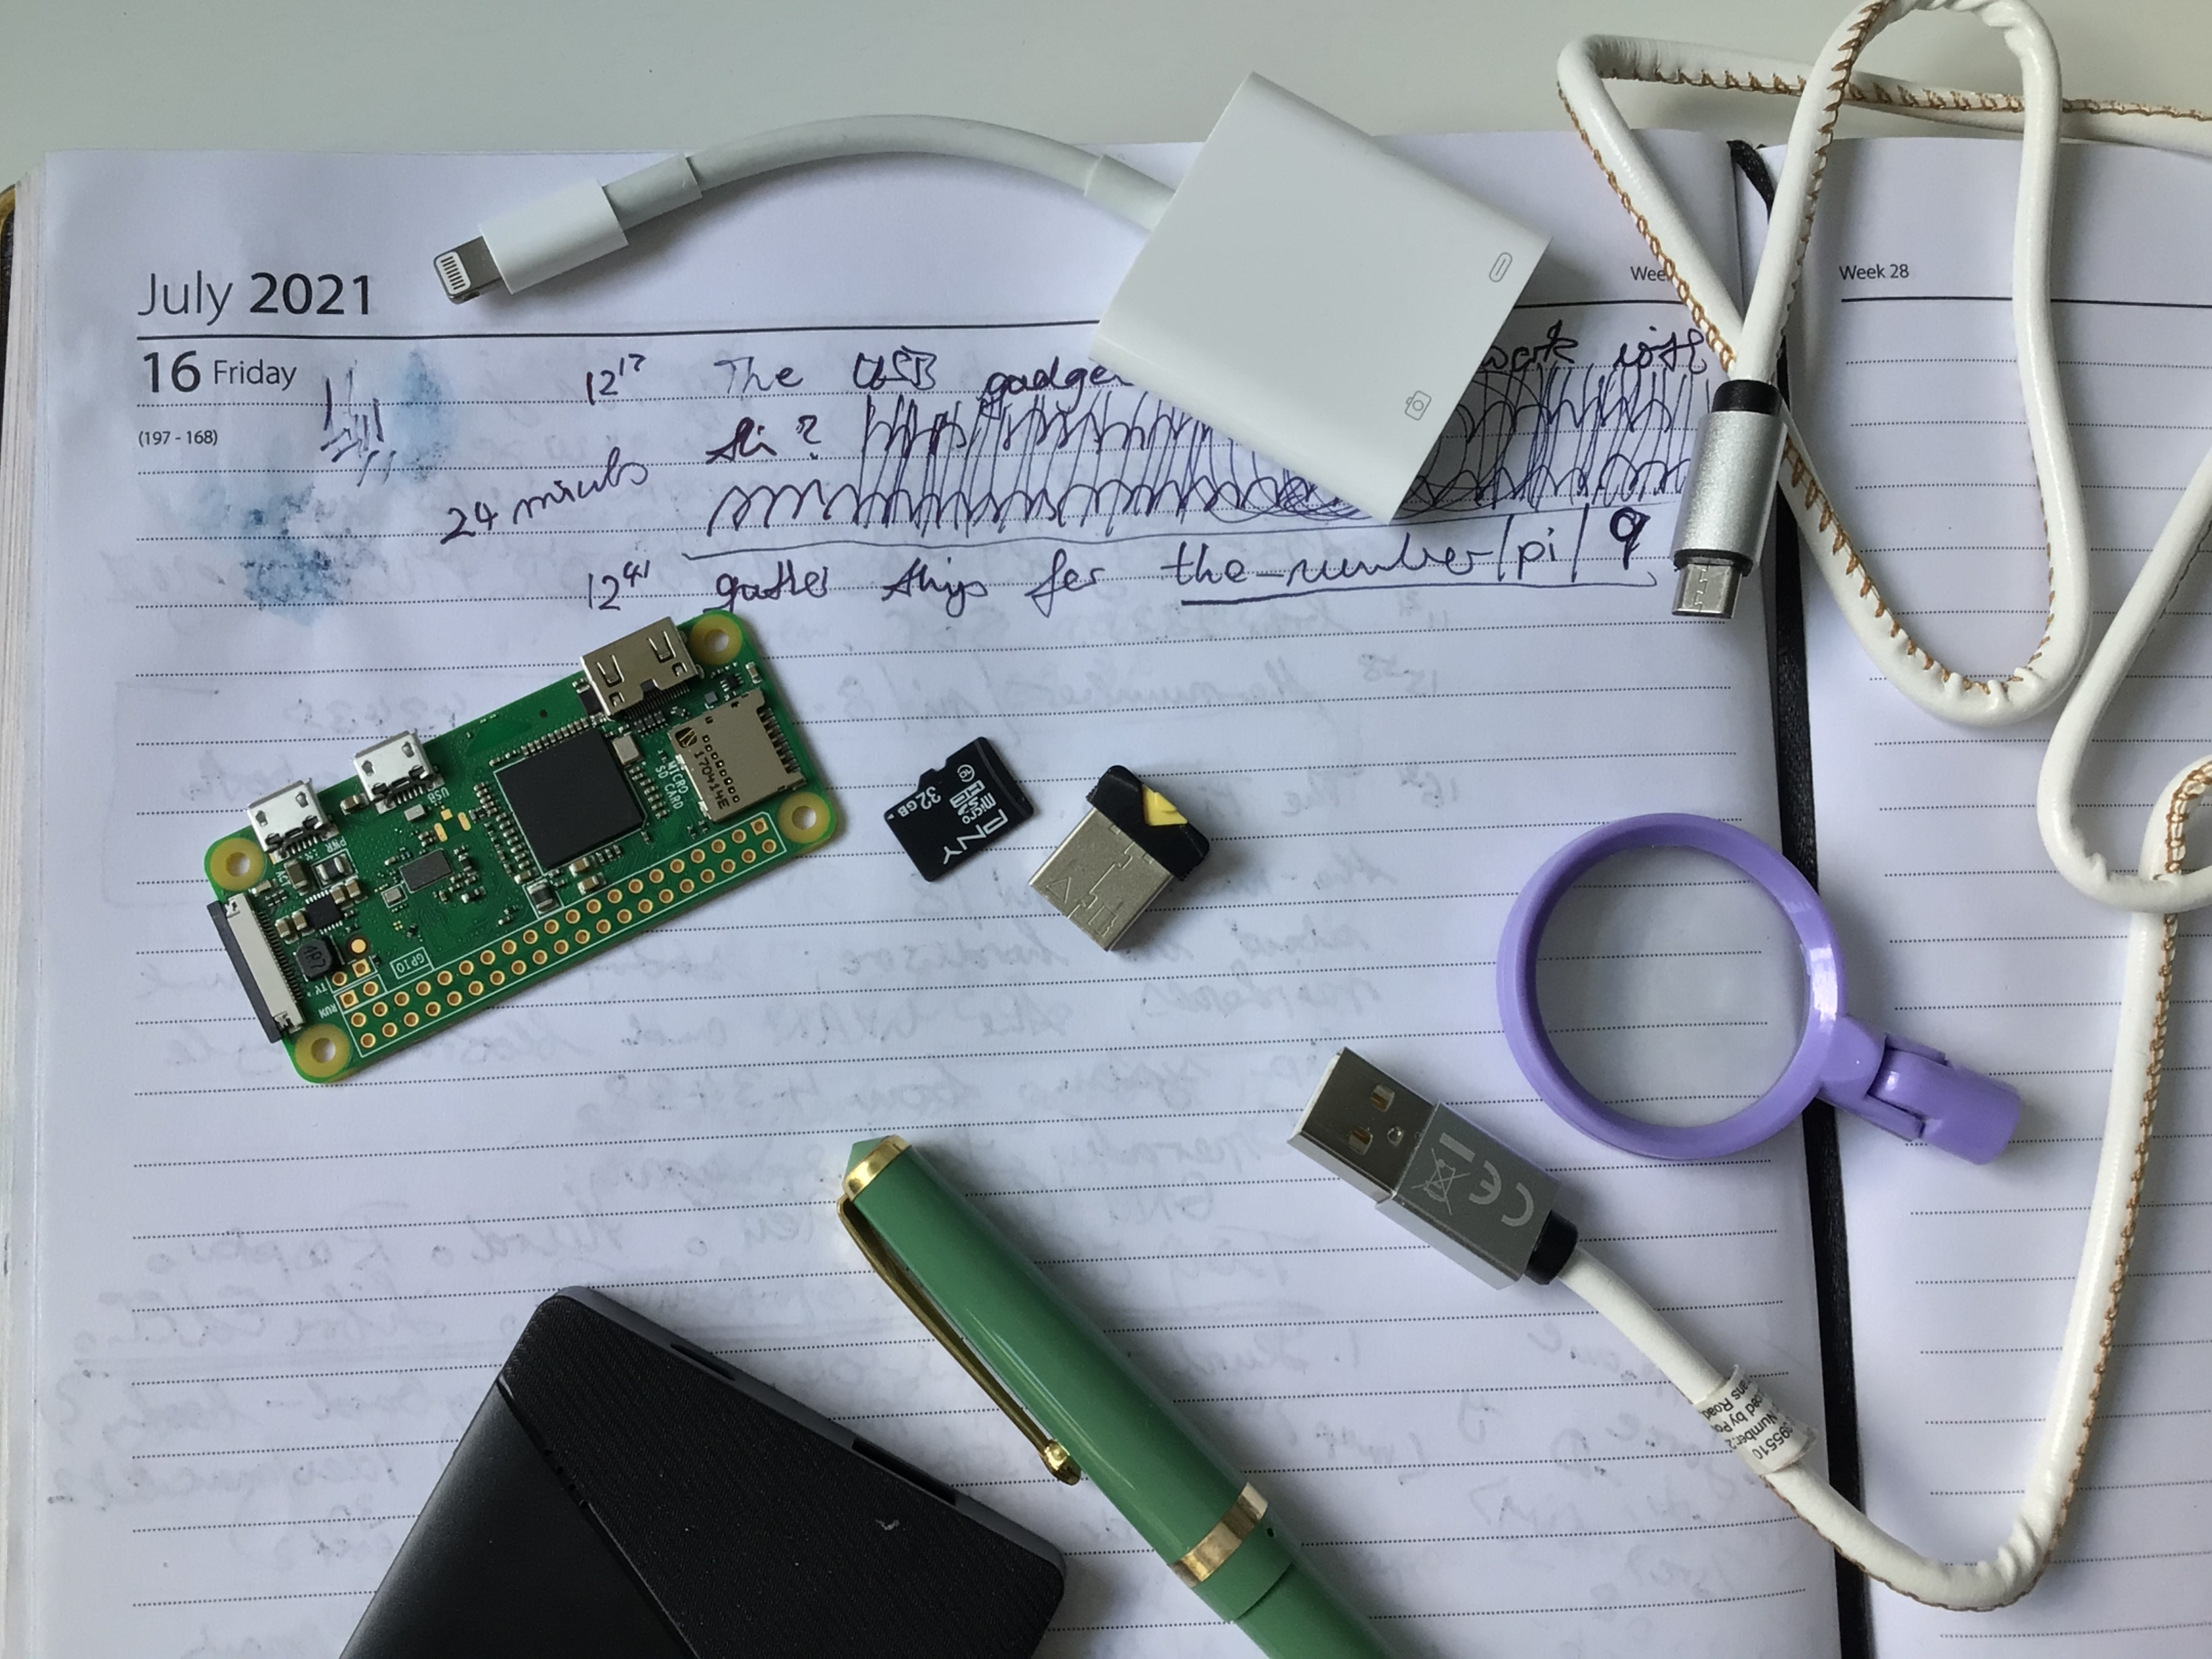
\includegraphics[width=.9\linewidth]{./i/5.jpg}
\subsection{SD memory for this iPad to change}
\label{sec-1-3}

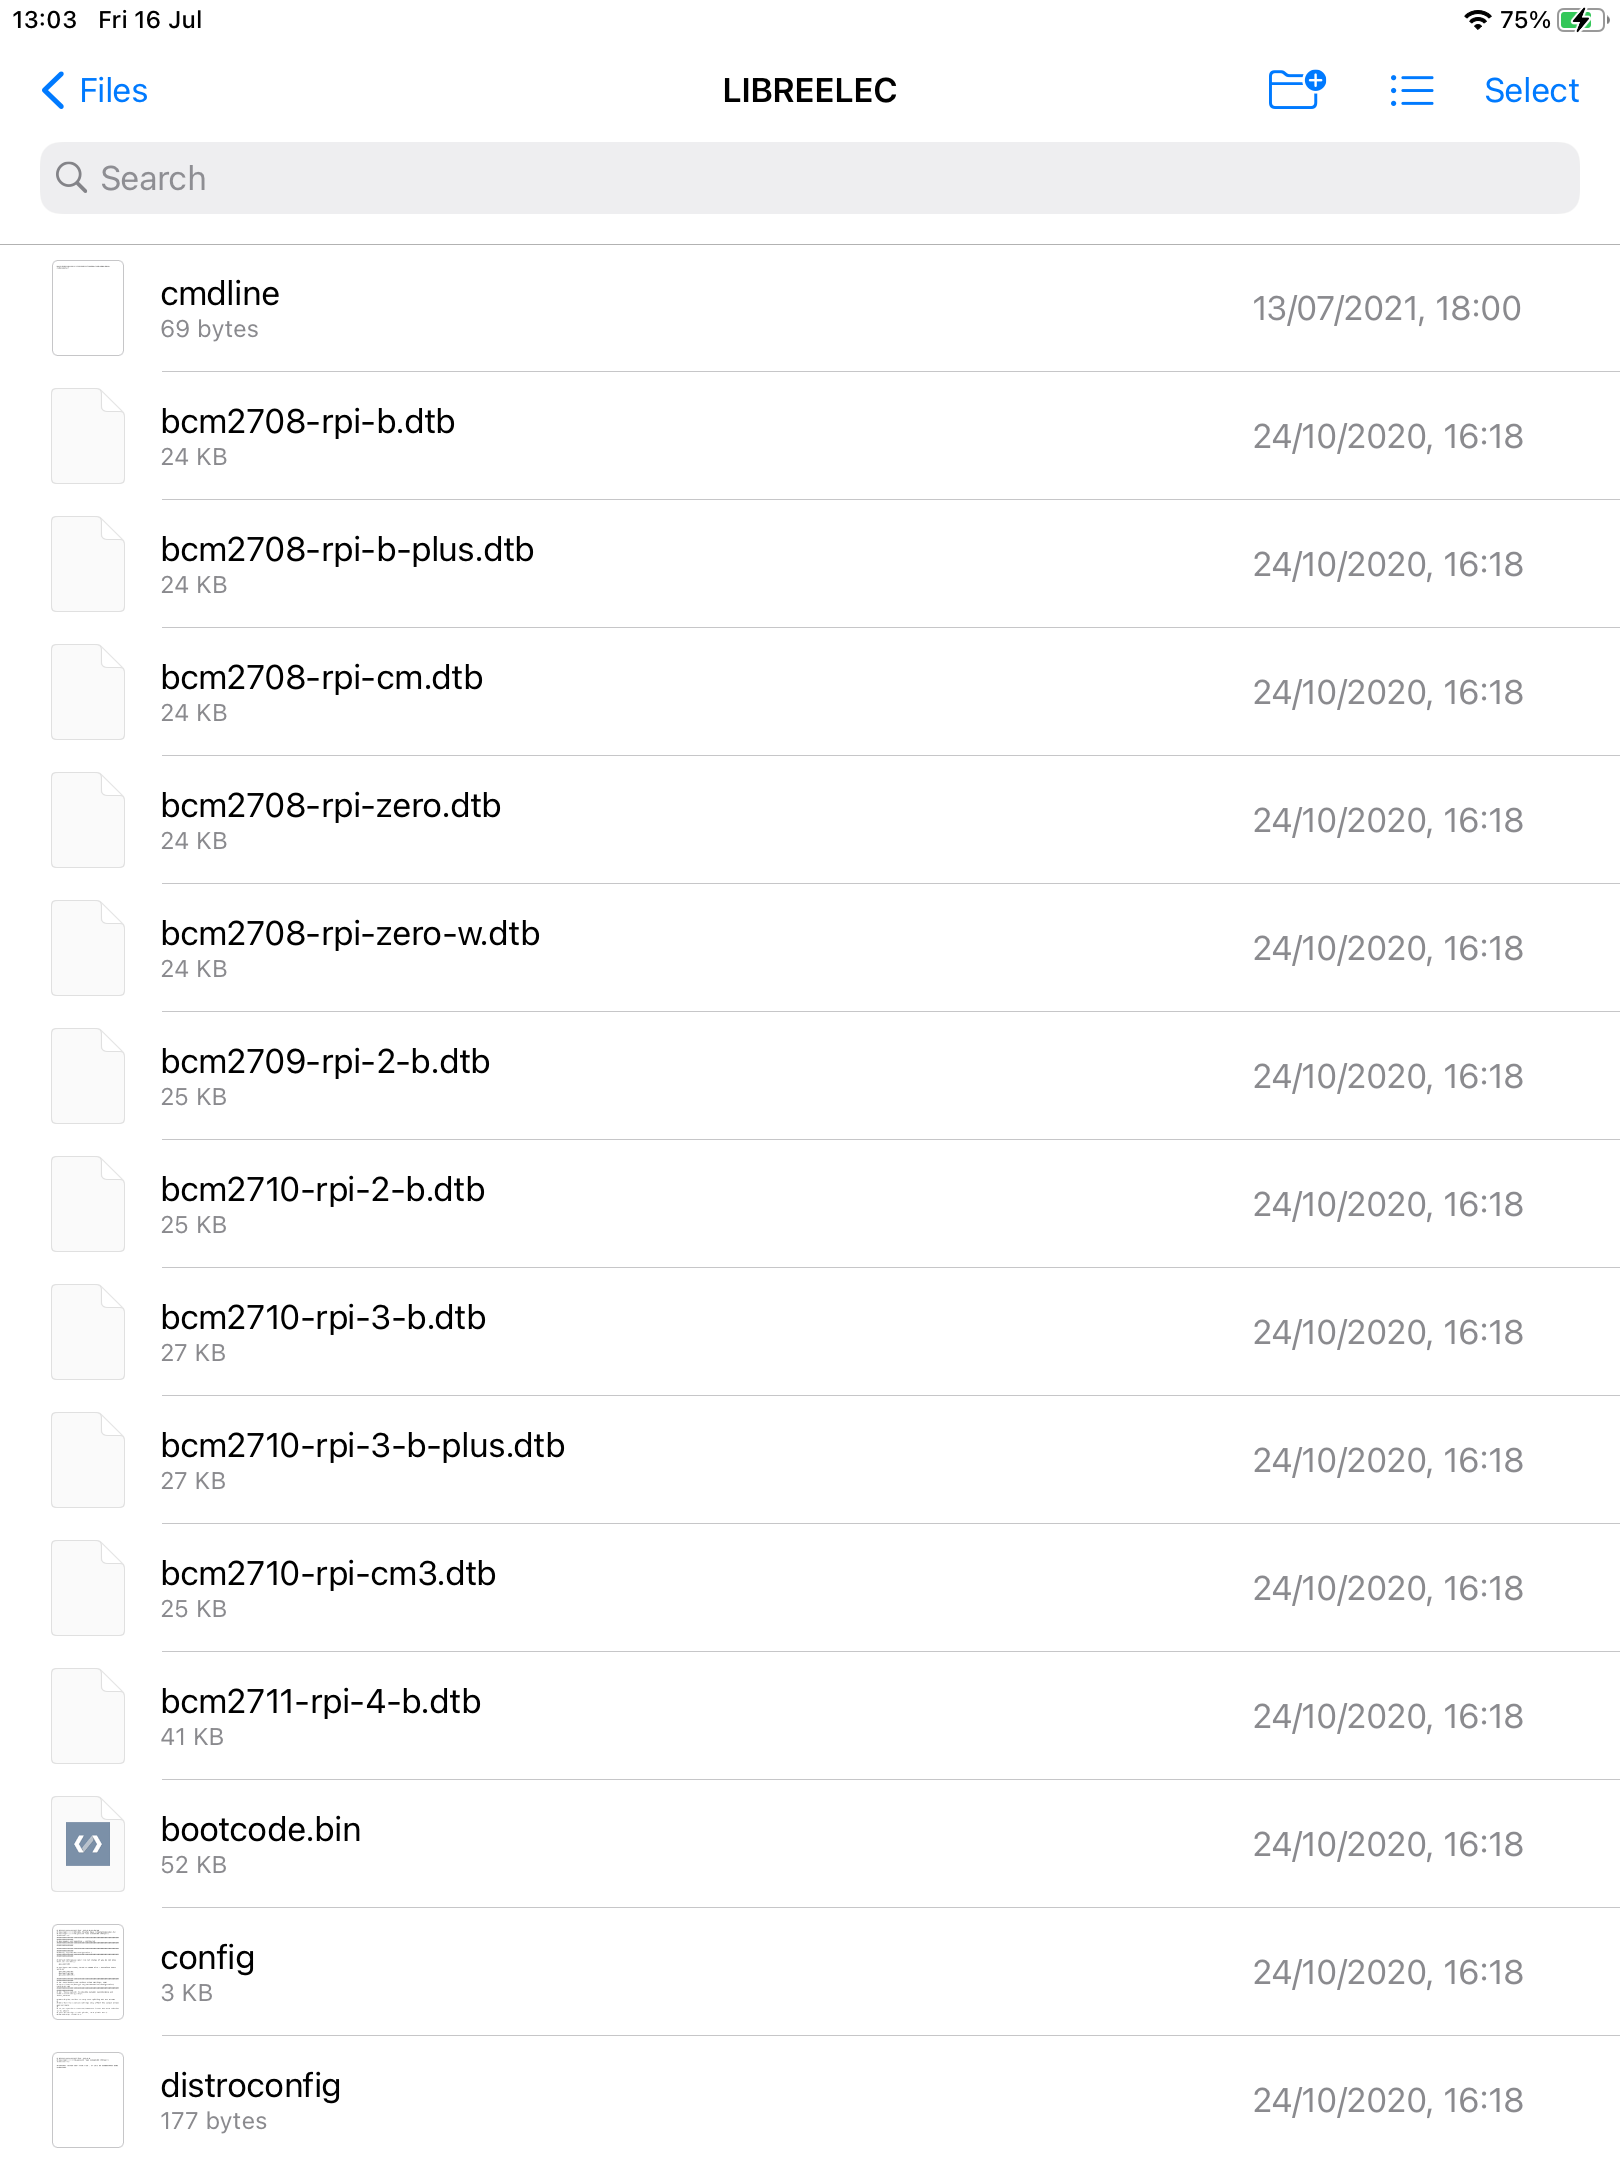
\includegraphics[width=.9\linewidth]{./i/6.png}
\subsection{Here, we pause, as more needs to be}
\label{sec-1-4}

   here is the picture, so far
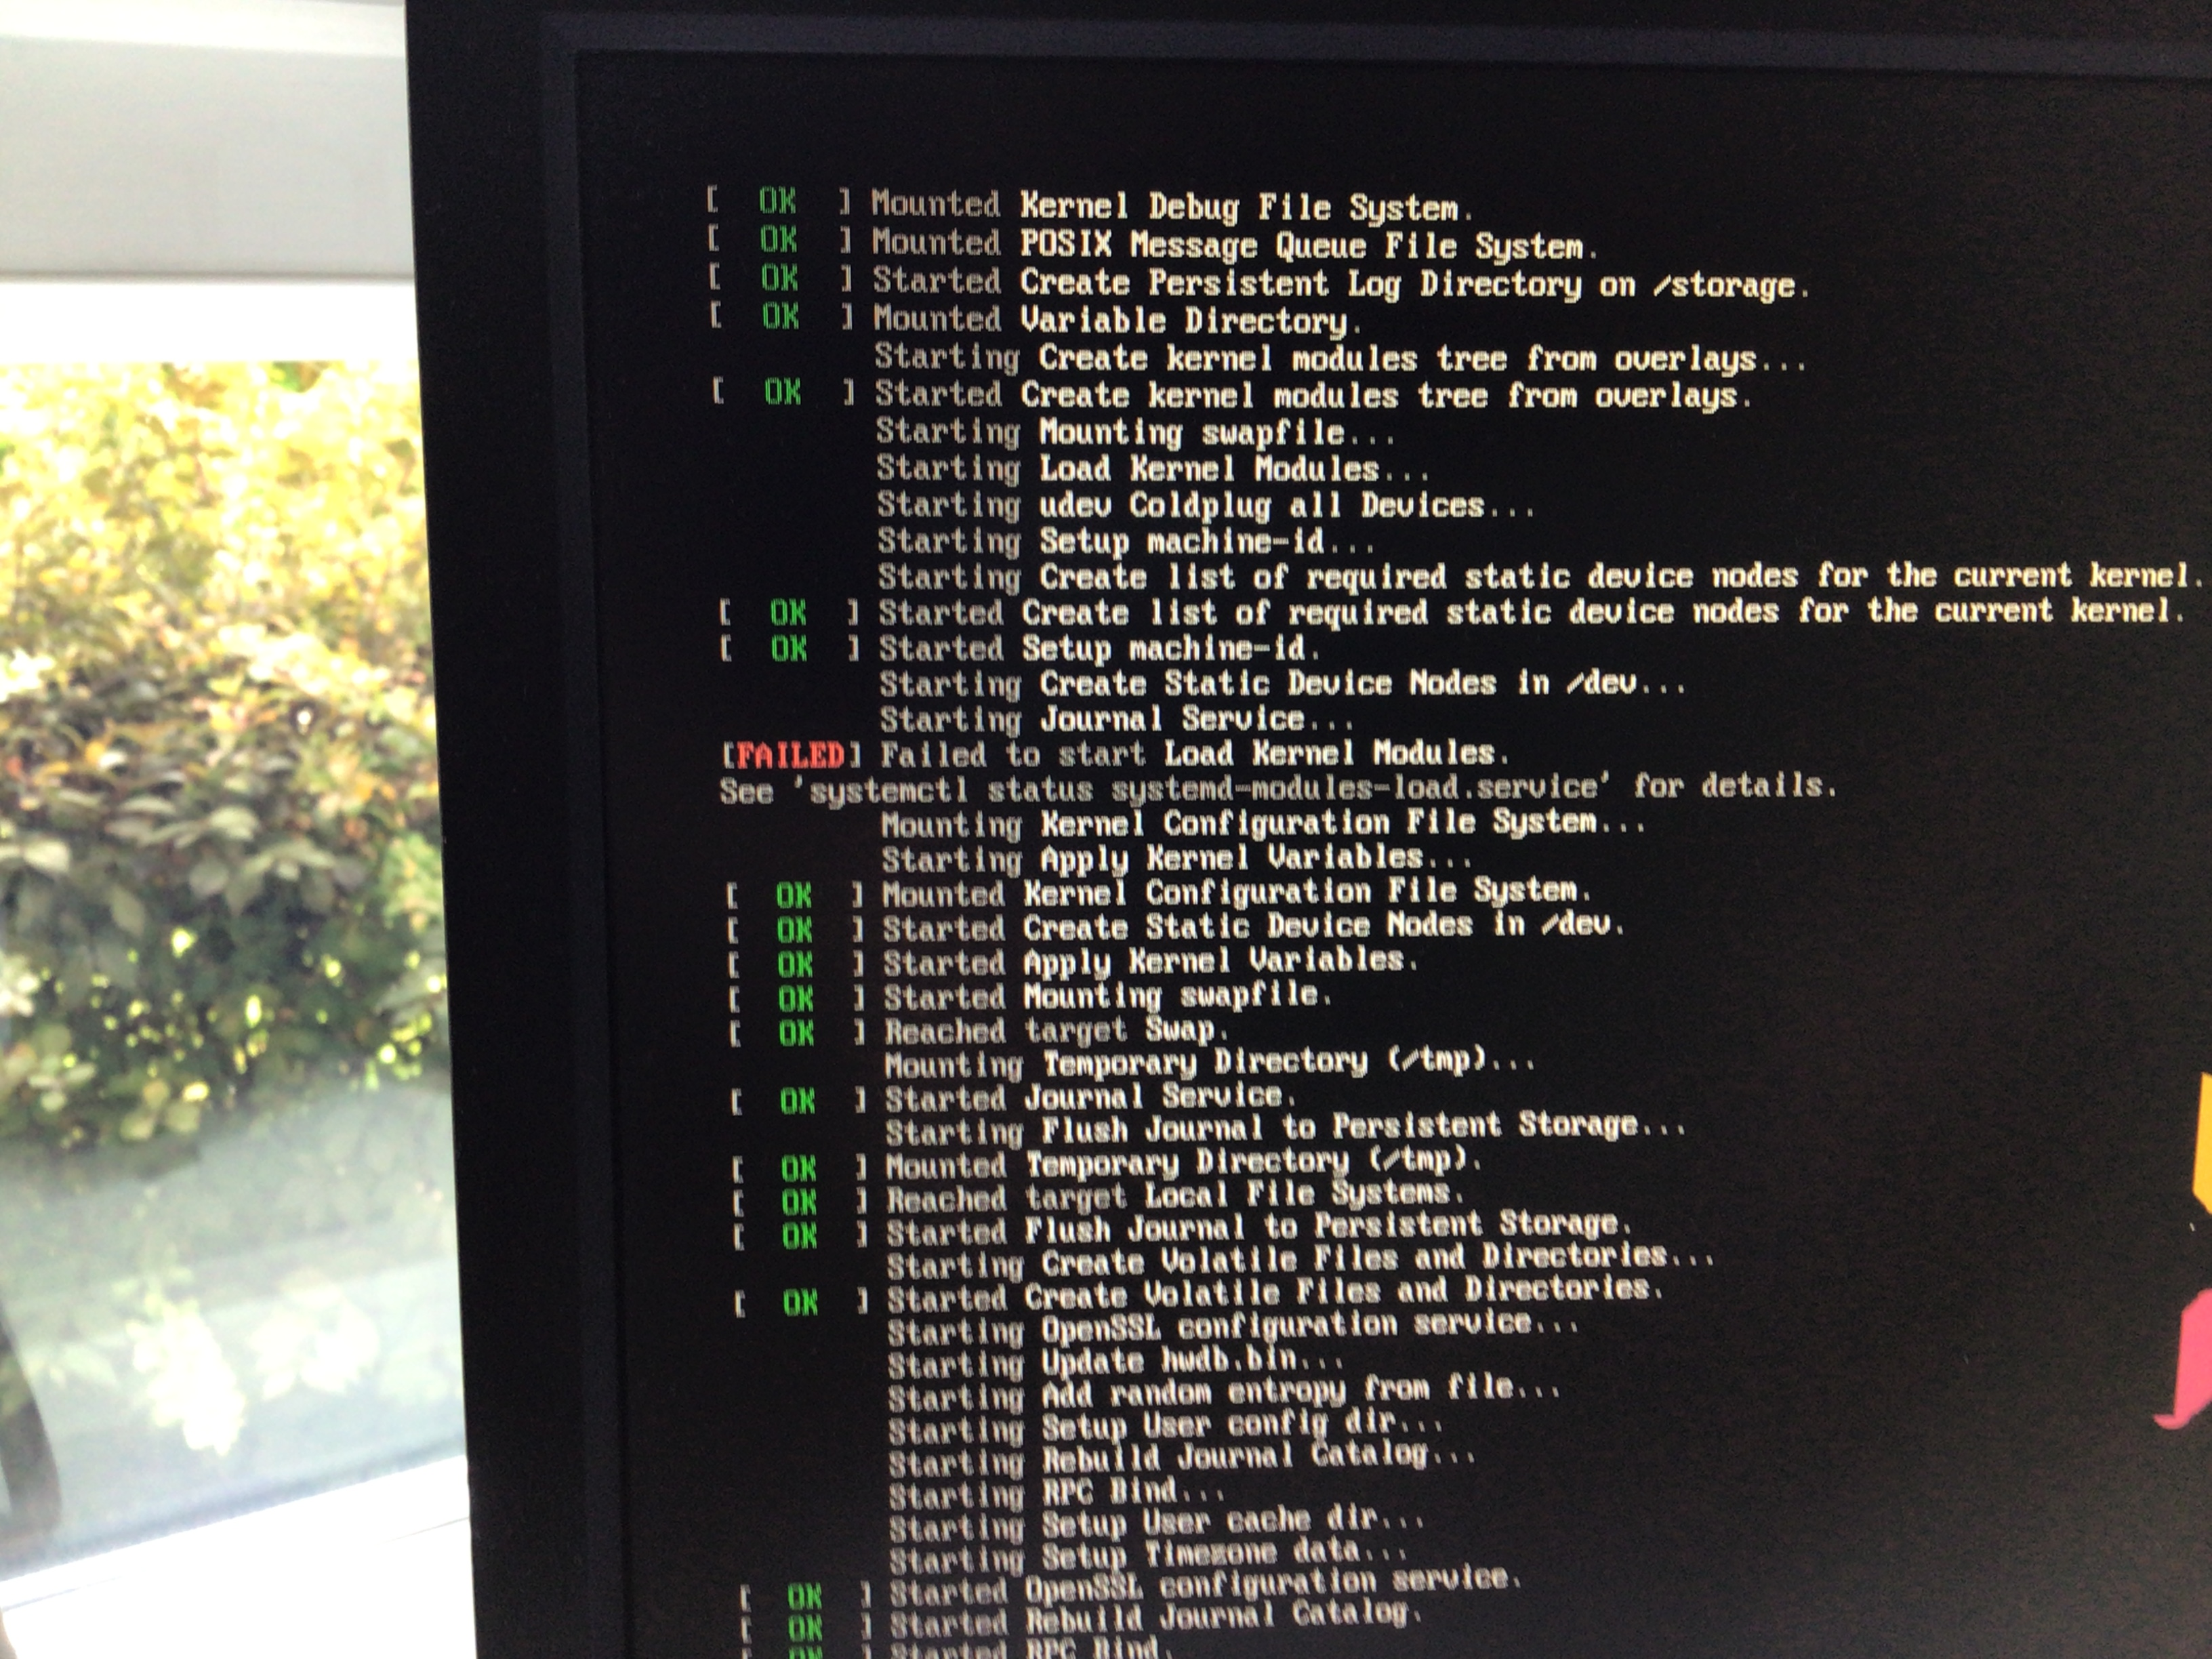
\includegraphics[width=.9\linewidth]{./i/e0.jpg}
\subsubsection{config.txt}
\label{sec-1-4-1}

\begin{verbatim}
 dtoverlay=dwc2
\end{verbatim}
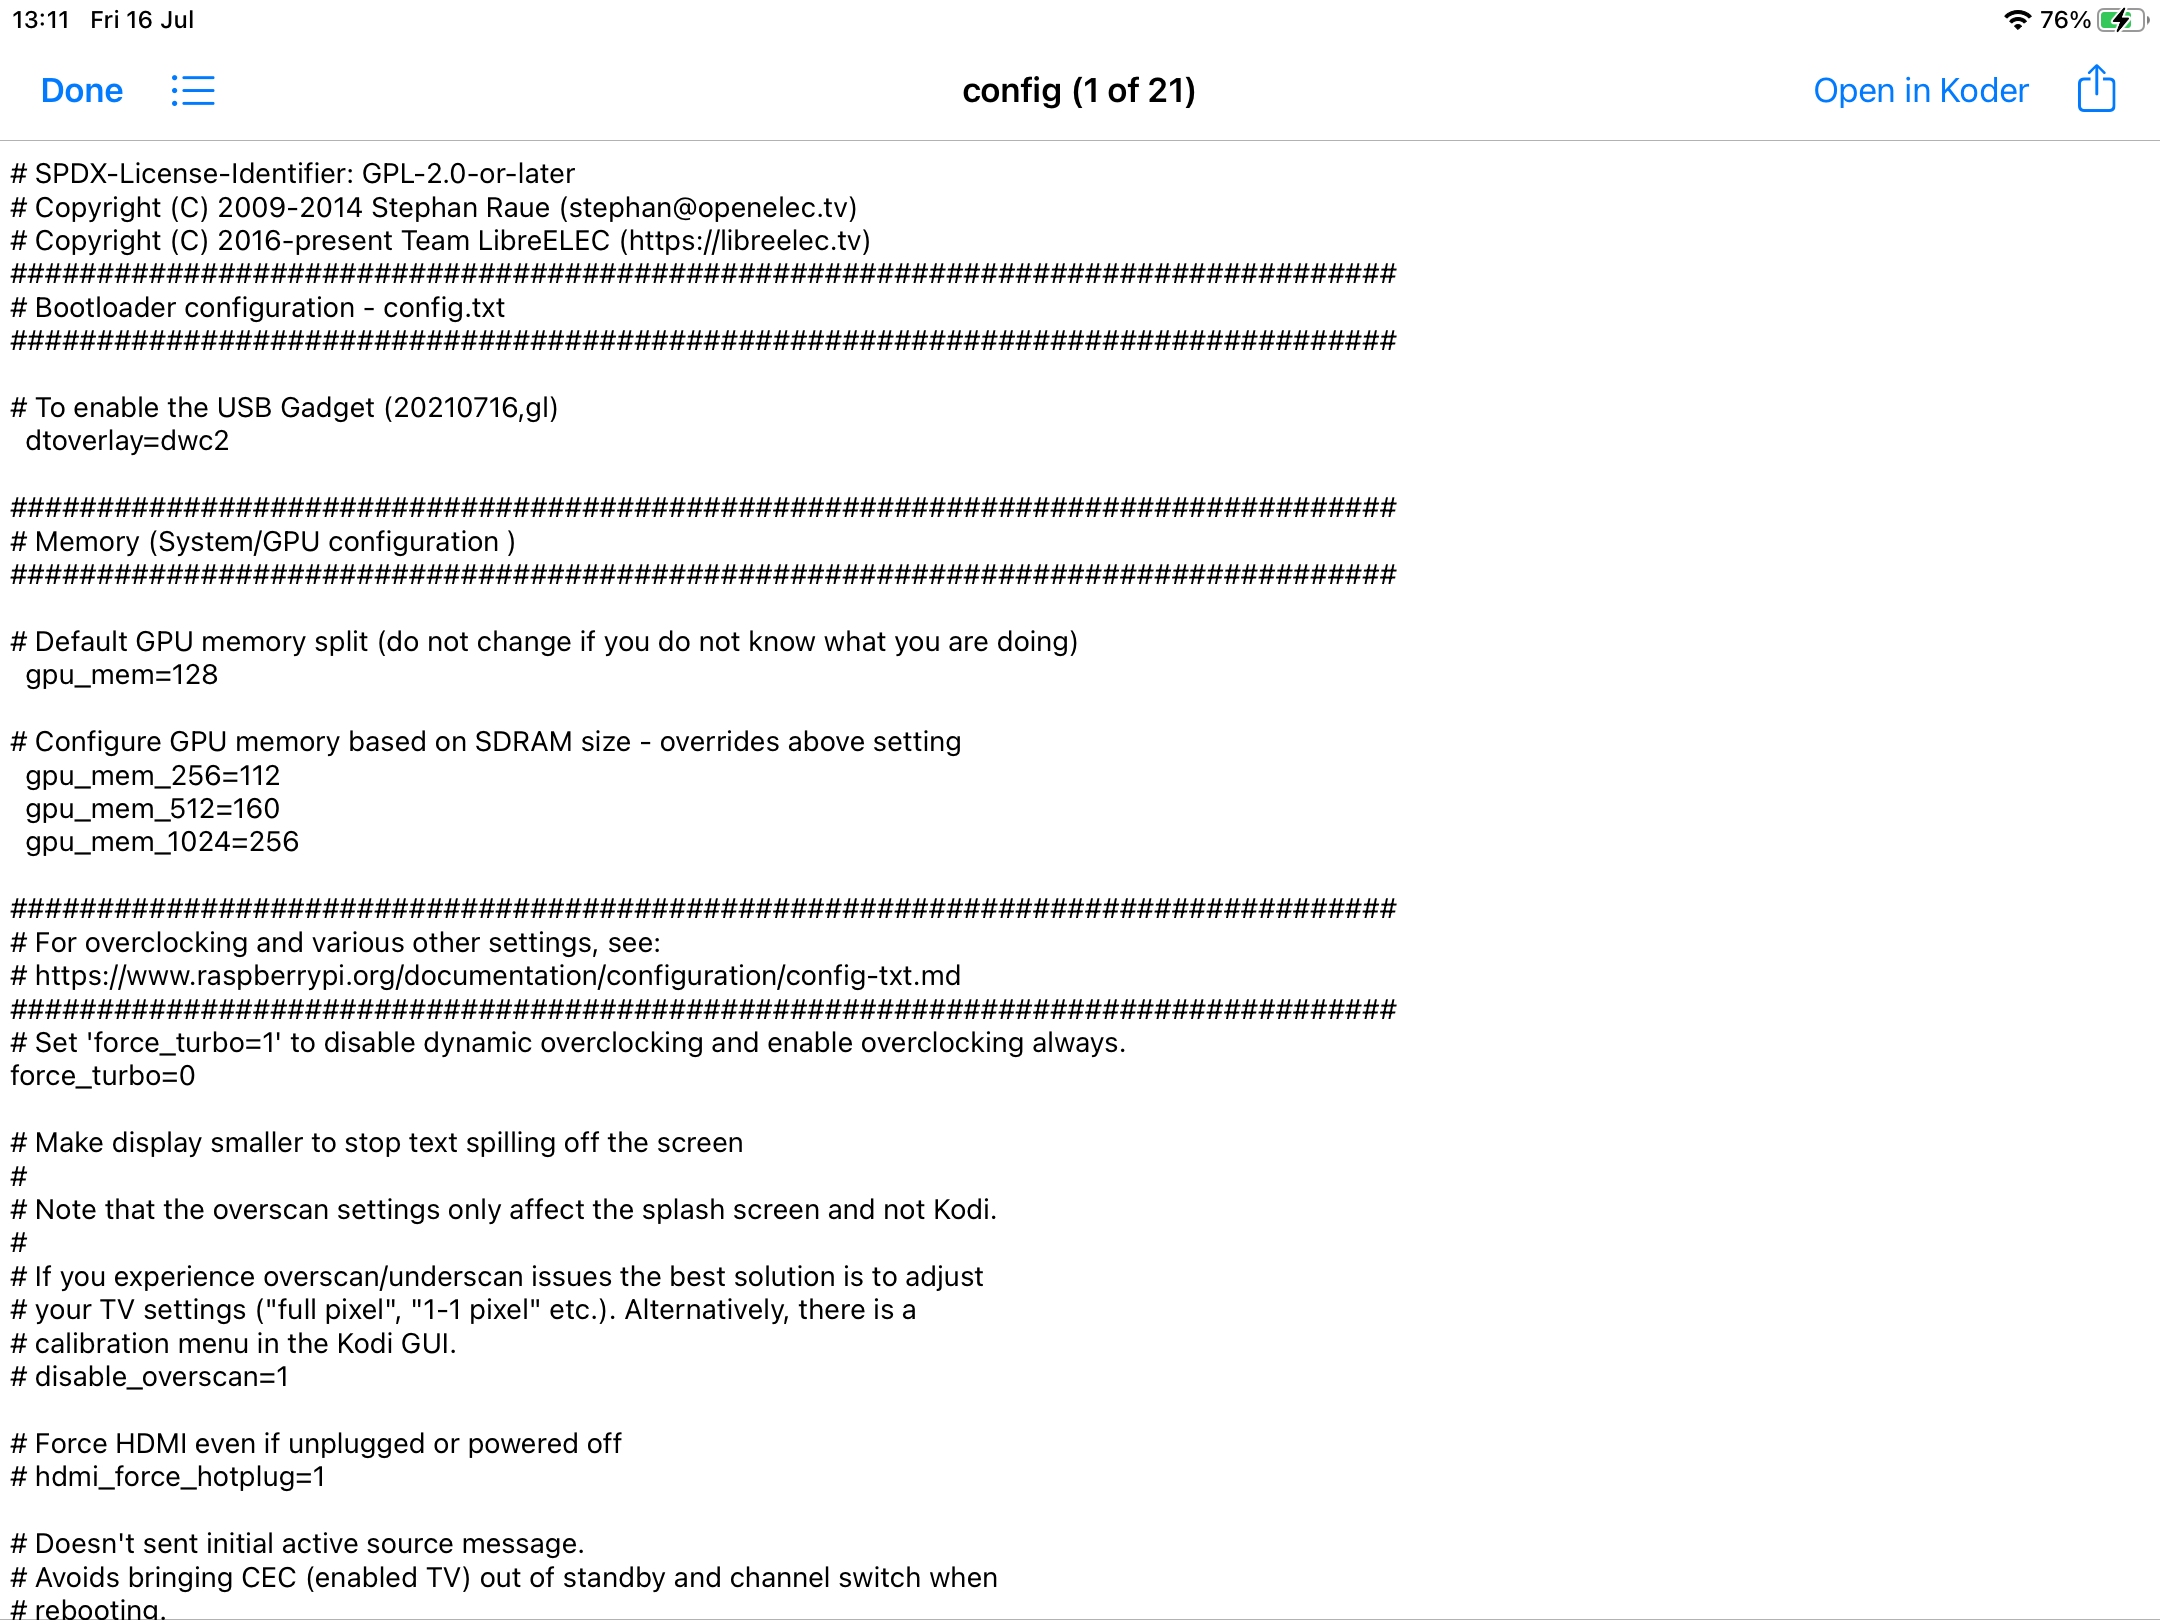
\includegraphics[width=.9\linewidth]{./i/8.png}
\subsubsection{cmdline.txt}
\label{sec-1-4-2}

(after rootwait, exactly one space)
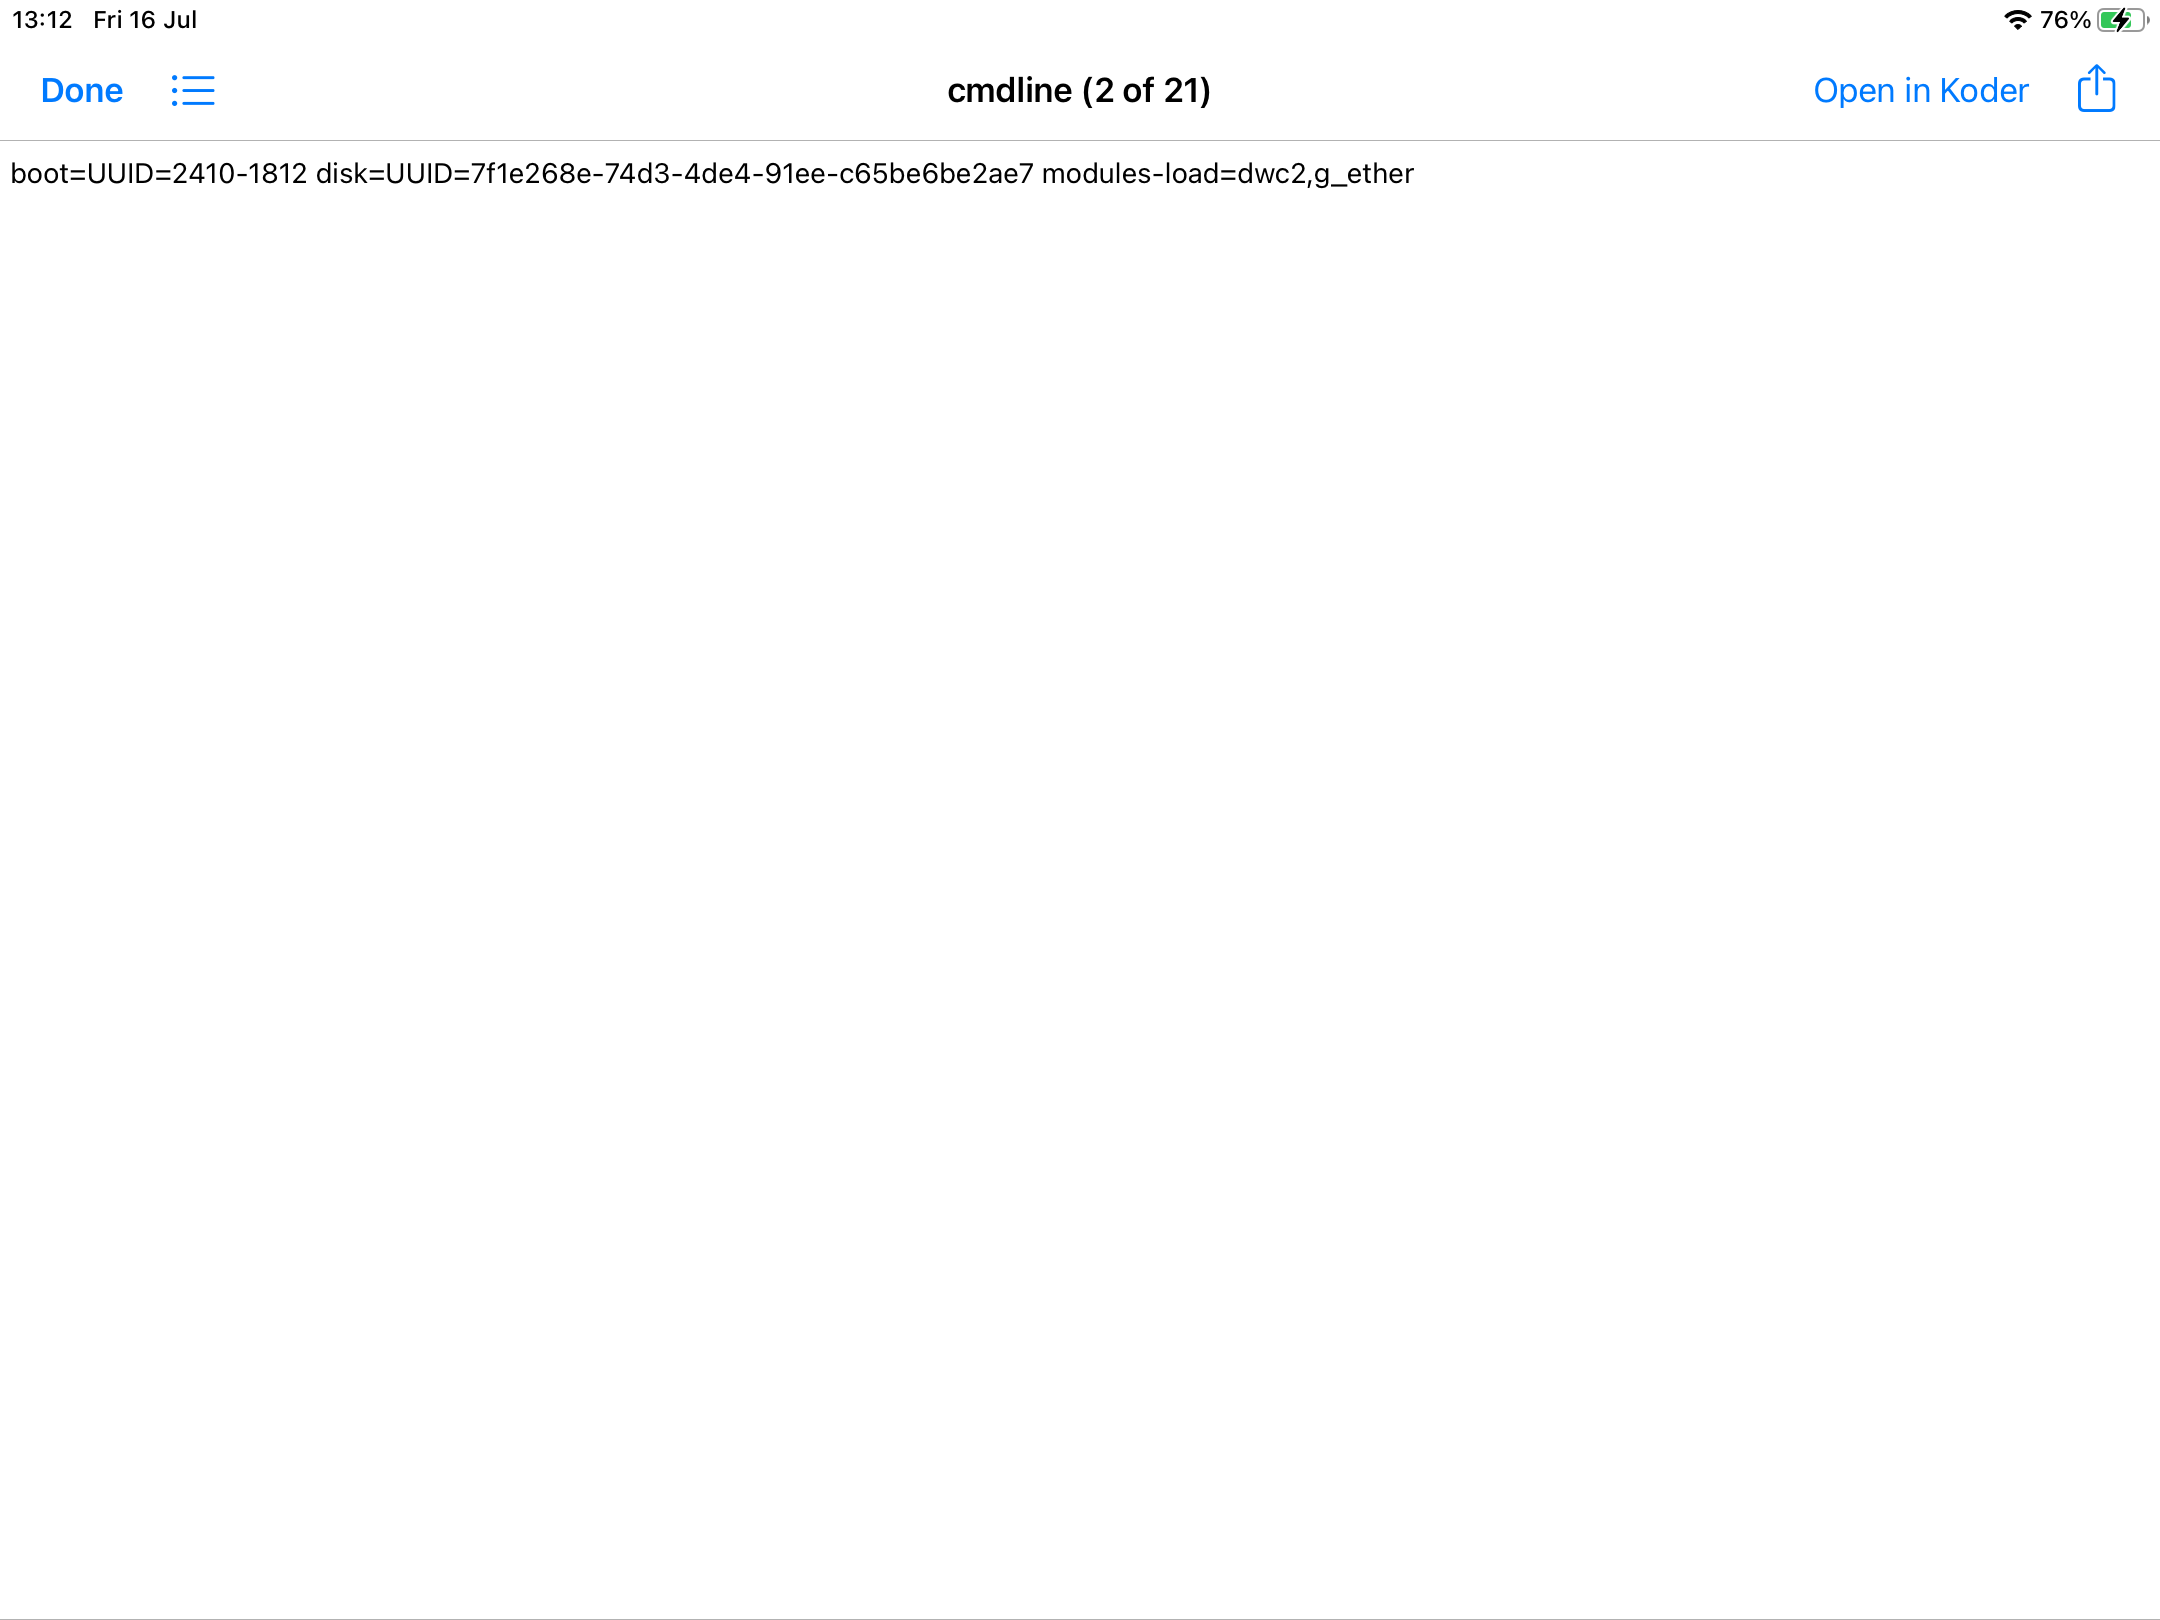
\includegraphics[width=.9\linewidth]{./i/7.png}
\begin{verbatim}
 modules-load=dwc2,g_ether
\end{verbatim}
\subsection{The Pi to boot}
\label{sec-1-5}

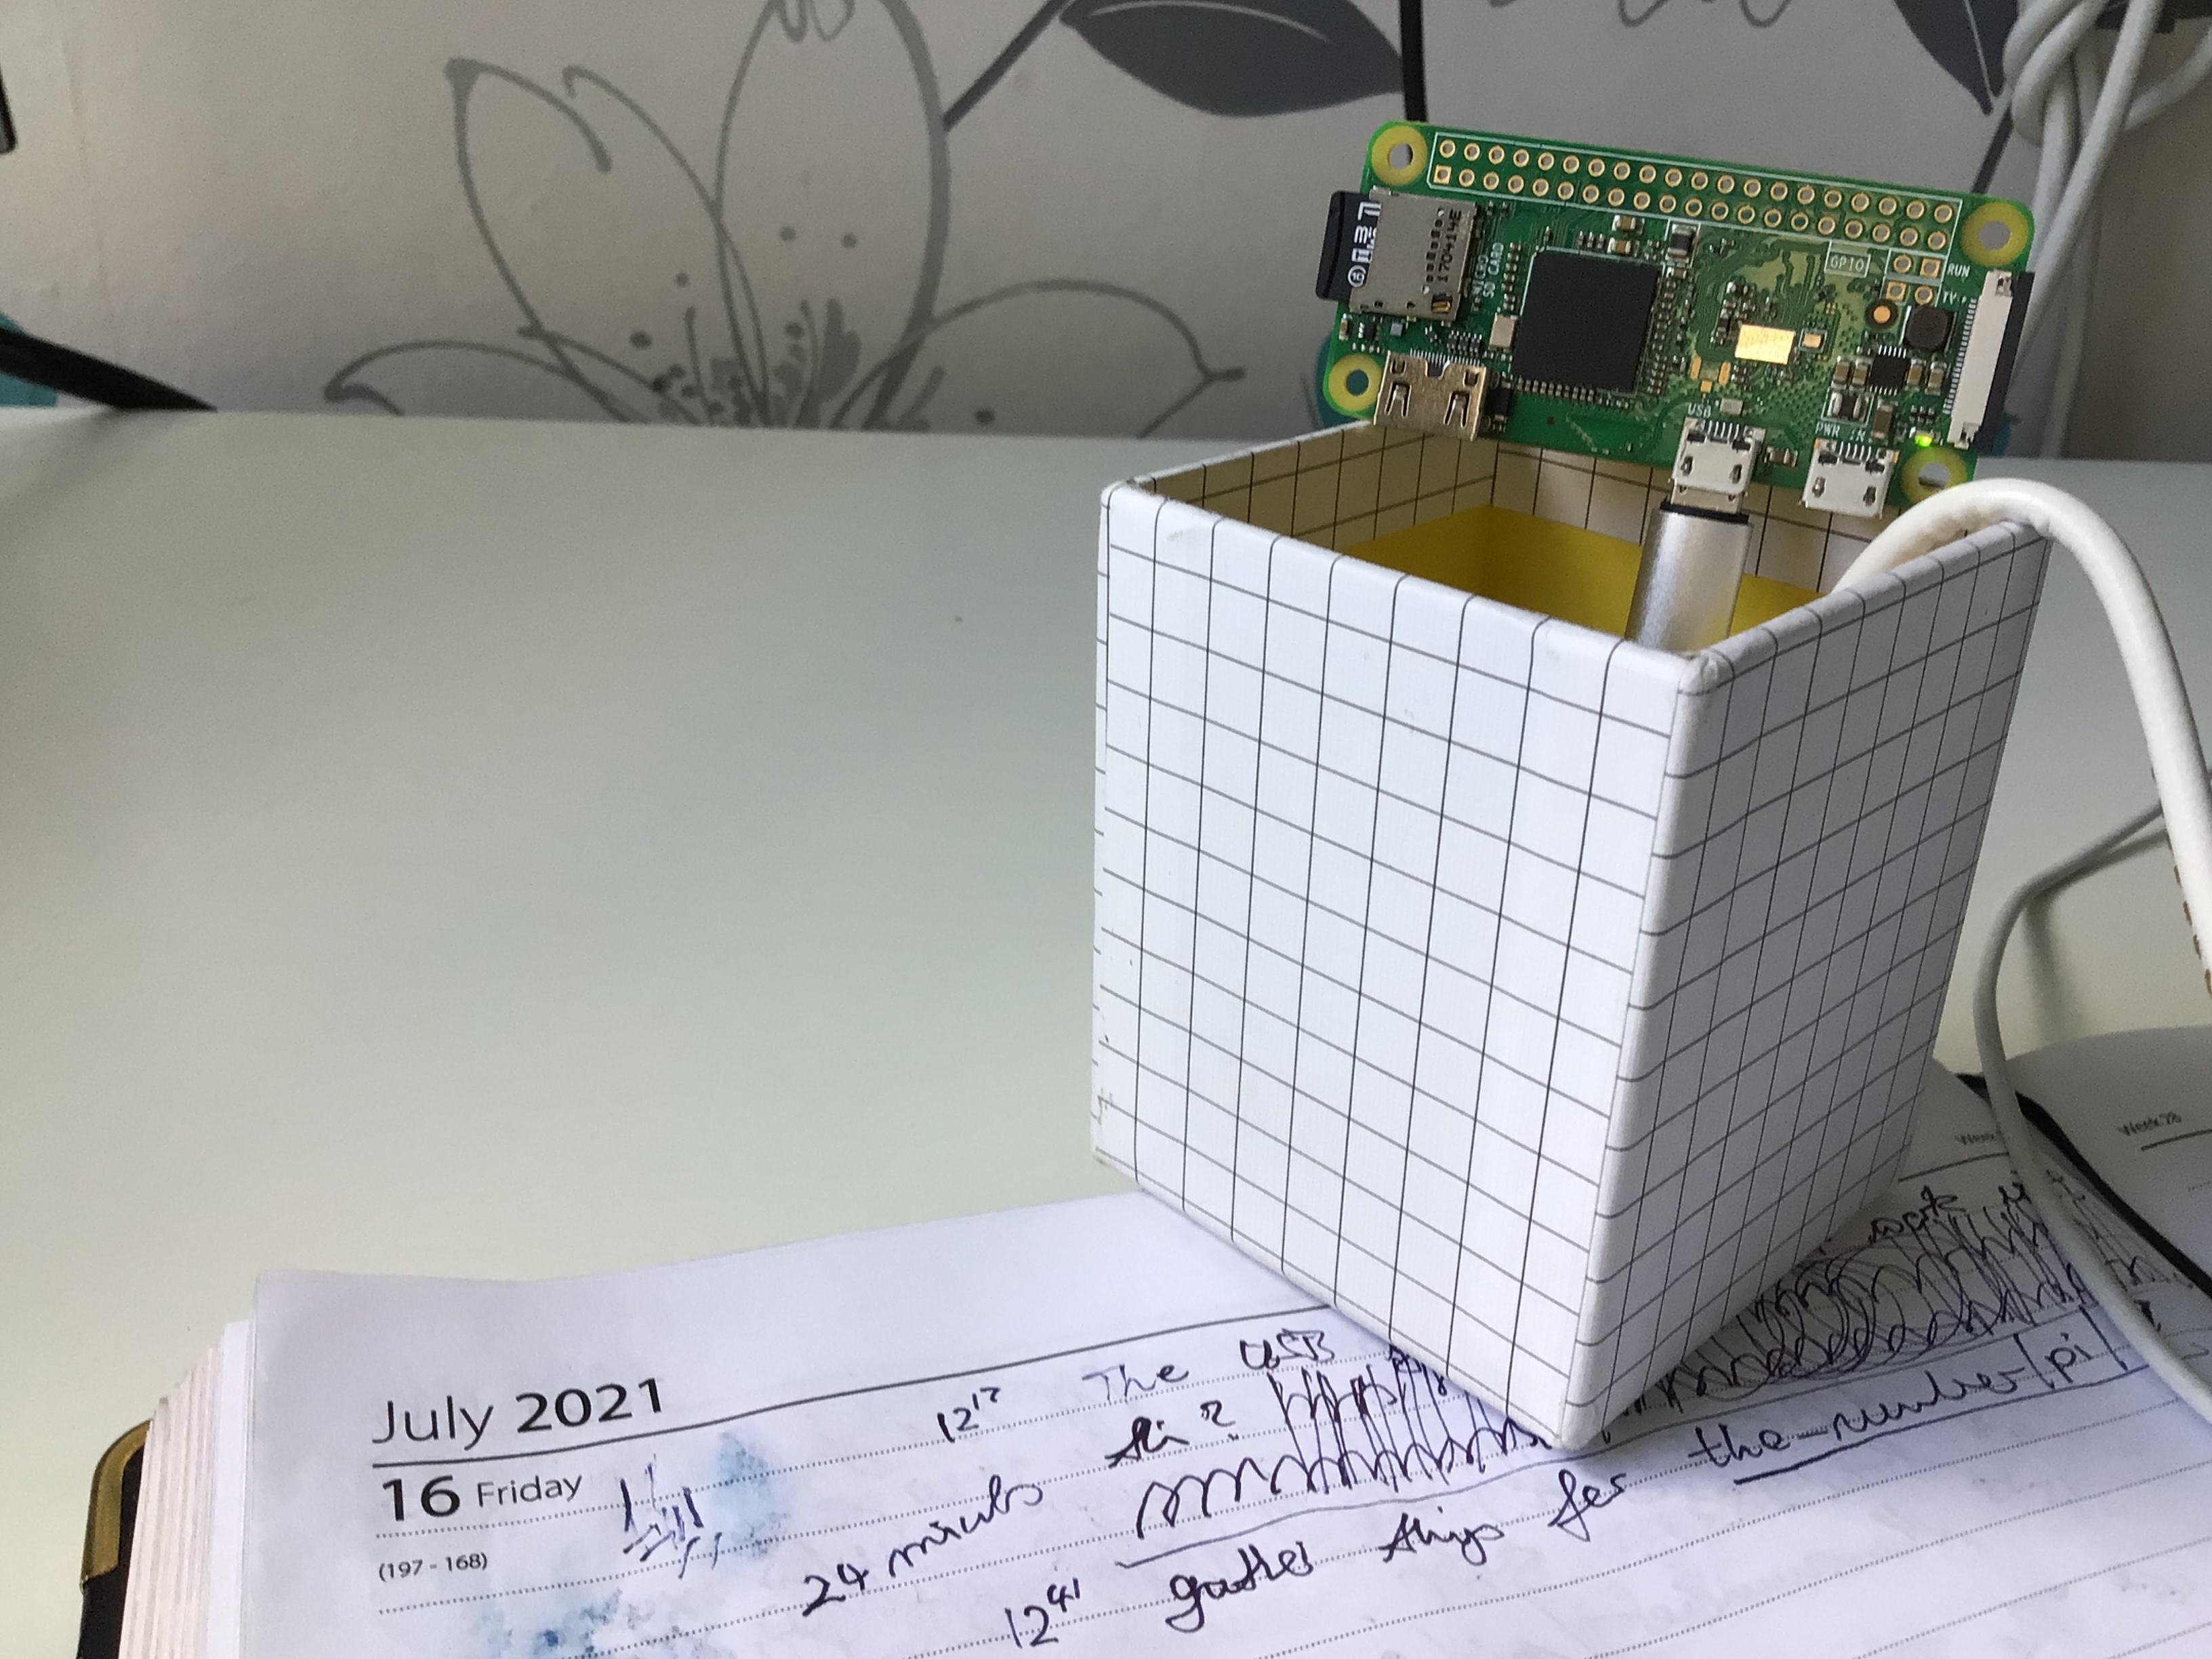
\includegraphics[width=.9\linewidth]{./i/1.jpg}
\subsection{The Pi Terminus}
\label{sec-1-6}
\subsubsection{The address}
\label{sec-1-6-1}

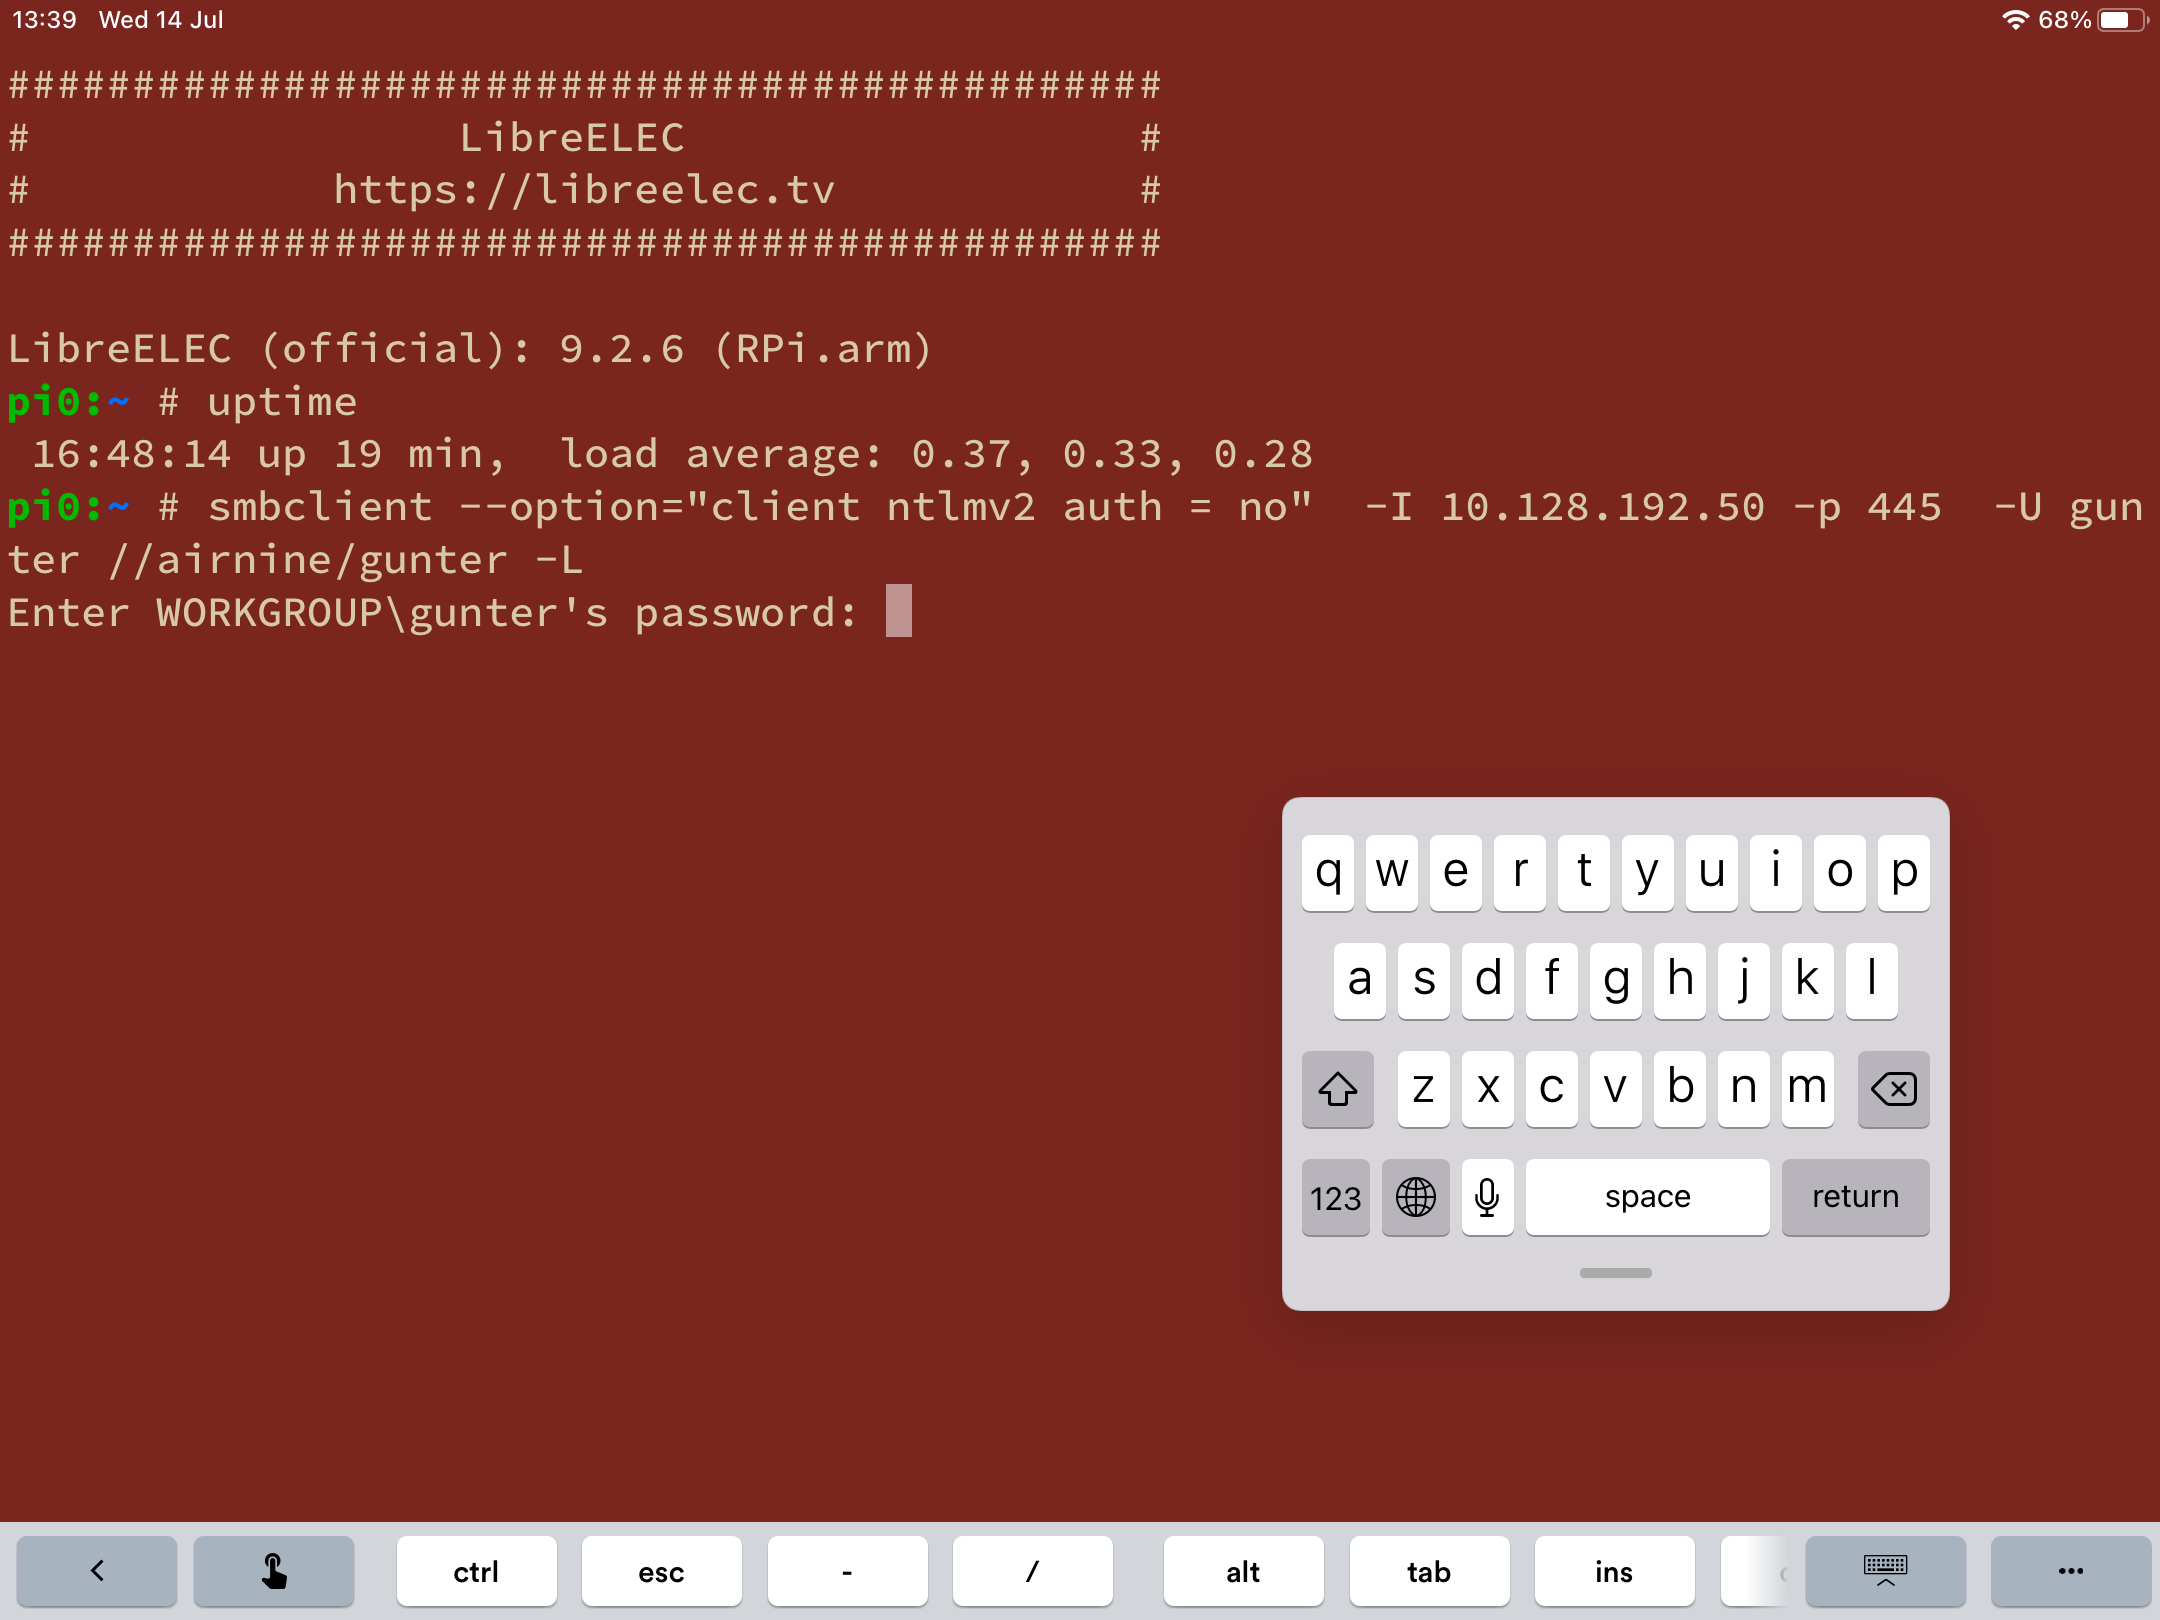
\includegraphics[width=.9\linewidth]{./i/2.png}
\subsubsection{The Pi on Air over USB}
\label{sec-1-6-2}

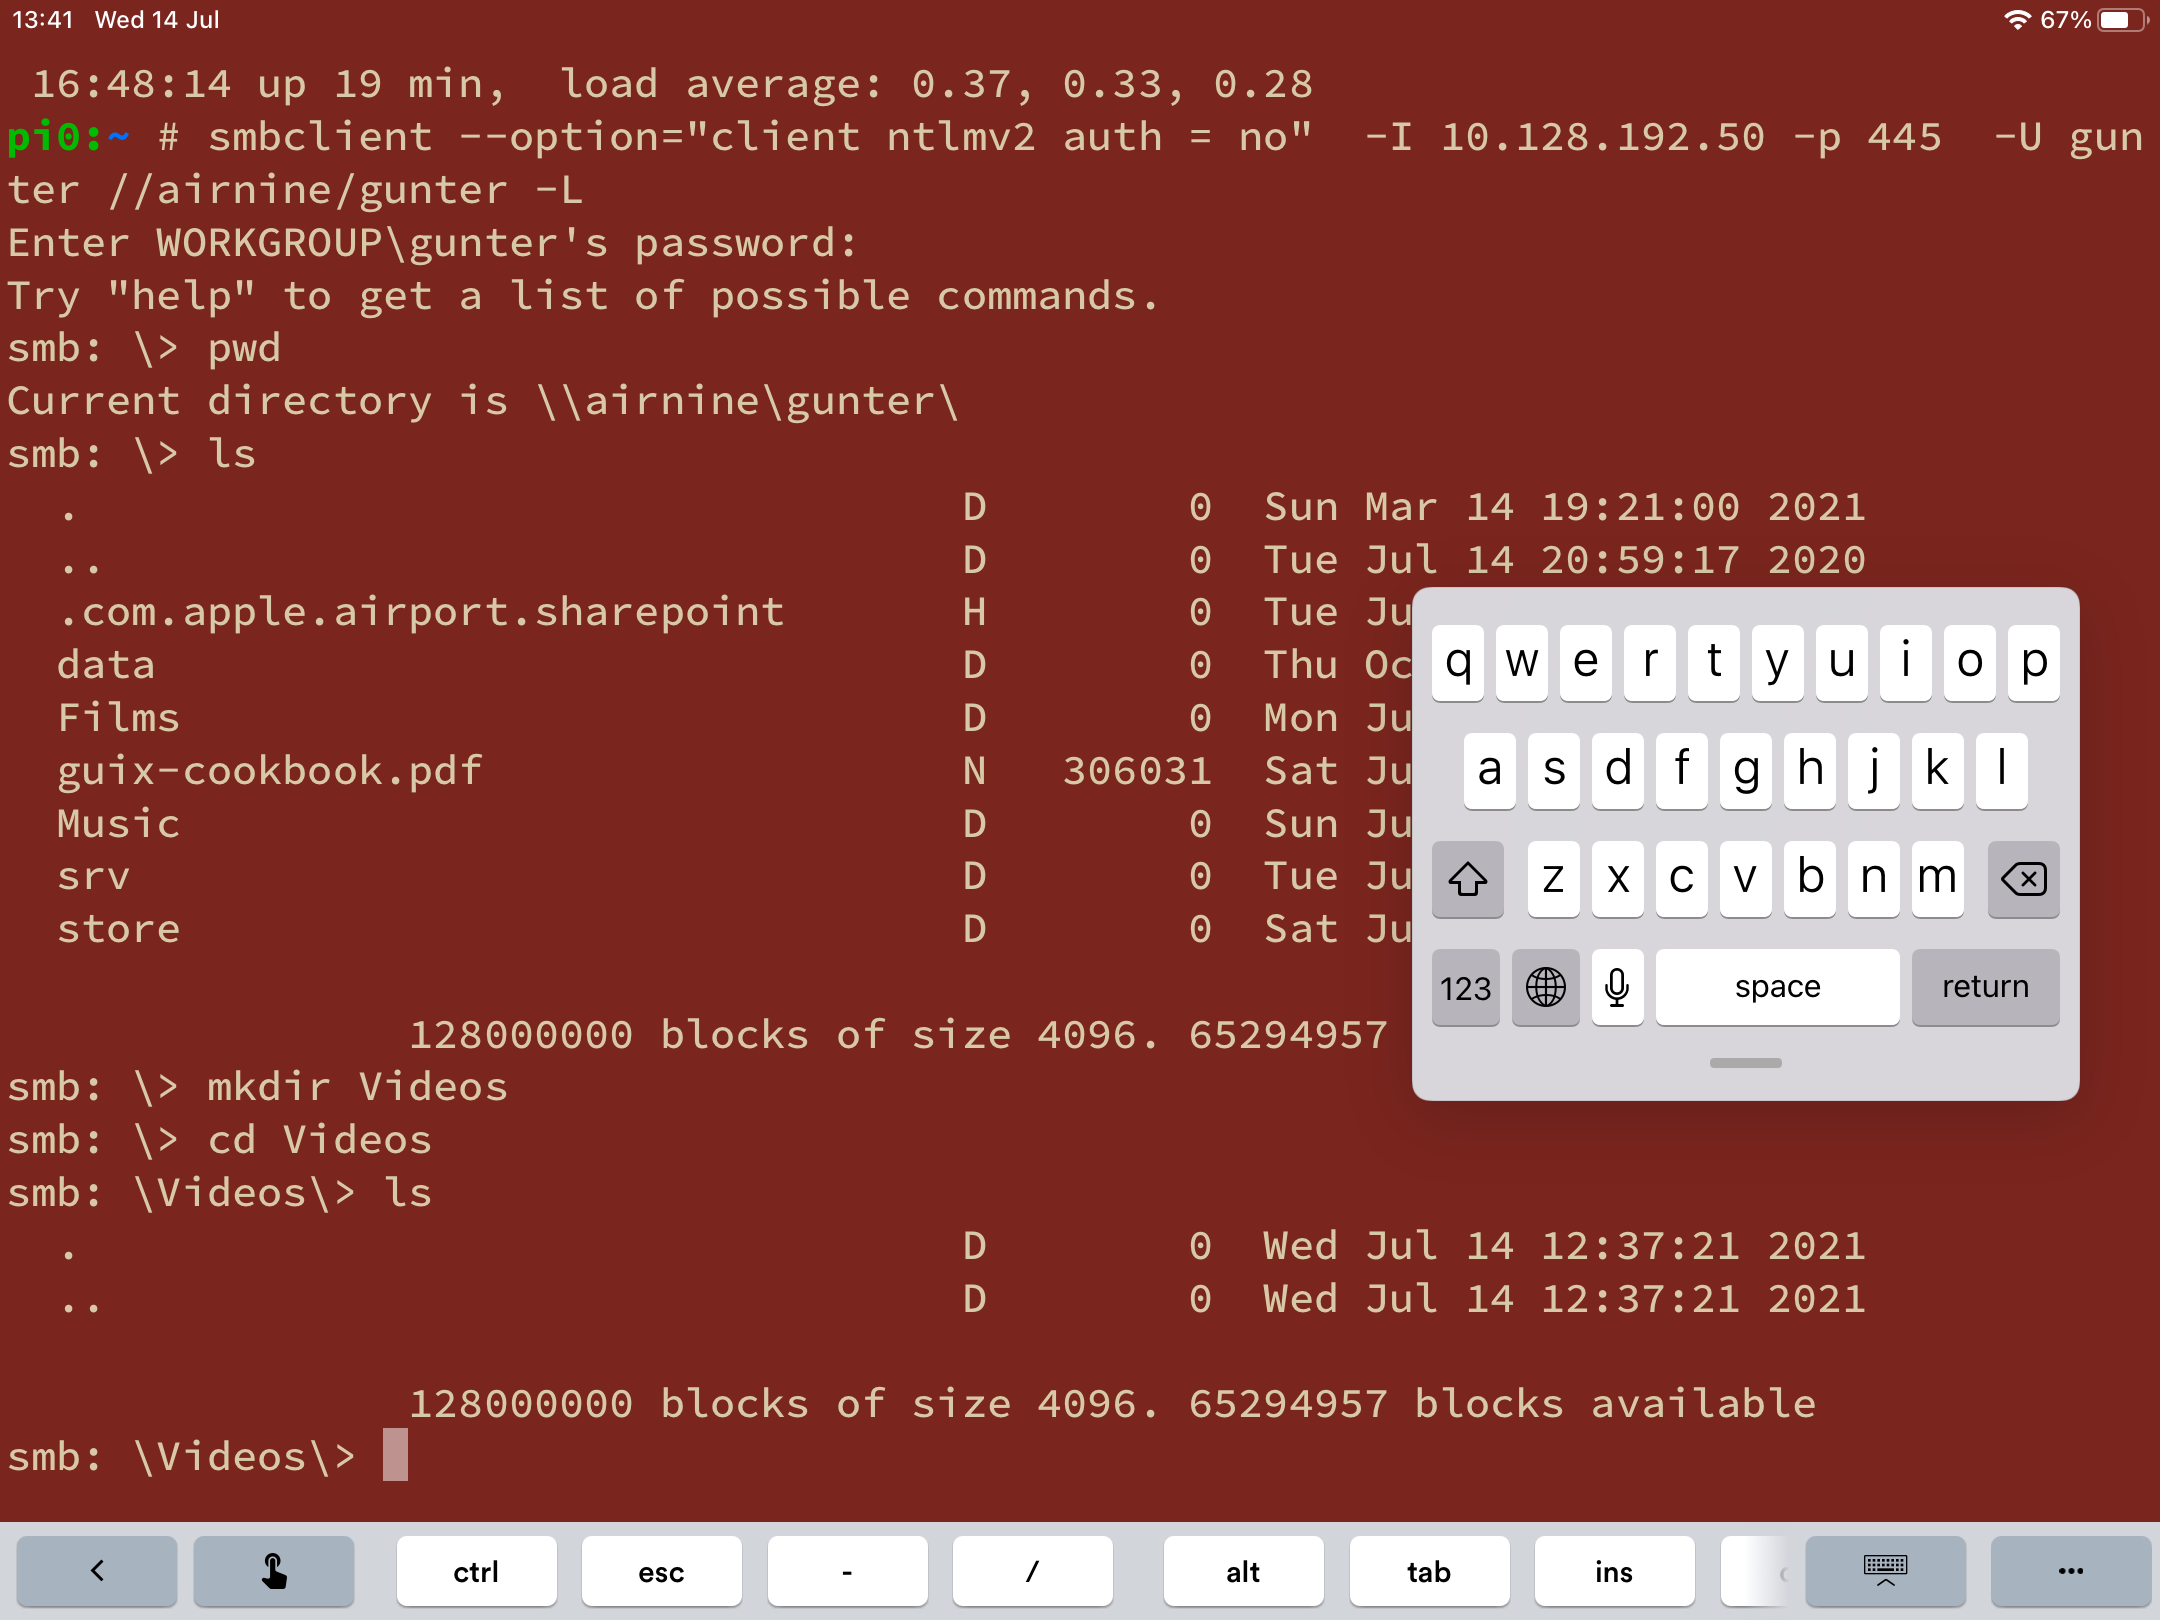
\includegraphics[width=.9\linewidth]{./i/3.png}

\end{document}
